\documentclass[12pt]{article}
\usepackage{amsmath}
\setlength{\jot}{2ex}
\usepackage{mathrsfs}
\usepackage{graphicx}
\usepackage{wrapfig}
\usepackage{booktabs}
\usepackage[letterpaper, margin=1in]{geometry}
\usepackage{indentfirst}
\usepackage{fancyhdr}
\usepackage [autostyle, english = american]{csquotes}
\MakeOuterQuote{"}
\renewcommand{\baselinestretch}{1.0}
\newcommand{\objects}[2]{%
  \leavevmode\vbox{\hbox{#1}\nointerlineskip\hbox{#2}}%
}
\title{Lab 6 \\ Design of Finite State Machines}
\author{Qadis Chaudhry}
\date{May 7, 2021}
\begin{document}
\maketitle
    \par This lab deals with the design of finite state machines and in this
    instance, the machine is a controller responsible for the operation of an
    elevator.  There are two inputs and the two outputs which change based on
    the state the machine resides in, as well as the inputs given by the user.
    This allows for the user to control which floor the elevator will end up at
    based on the inputs they provide.
    \par In order to design any state machine, the equations of operation must
    be defined and the corresponding tables that are needed must be constructed
    from which, the machine can then be manifested. In this case there are four
    states, one for the elevator stopped at each of the three floors, and one
    for the elevator moving through the second floor. The state table can then
    be defined as:
    \begin{table}[h]
        \centering
        \begin{tabular}{cc}
            \toprule
            State & $Q_2 Q_1$ \\
            \midrule
            FLR1 & 00 \\
            FLR2 & 01 \\
            MOV2 & 10 \\
            FLR3 & 11 \\
            \bottomrule
        \end{tabular}
    \end{table}
    \par The inputs can also be defined as $R_1$ and $R_2$ and each of the
    possible combinations of these inputs corresponds to a specific request from
    the elevator.
    \begin{table}[h]
        \centering
        \begin{tabular}{cc}
            \toprule
            $R_1 R_2$ & Meaning \\
            \midrule
            00 & No request \\
            01 & Move to first floor \\
            10 & Move to second floor \\
            11 & Move to third floor \\
            \bottomrule
        \end{tabular}
    \end{table}
    \par With these tables the transition table for the controller can be
    interpreted. The transition table is what summarizes the main function of
    the machine and it will allow for the visualization of how the controller
    operates. This will also lead to the construction of the state diagram of
    the table and from there, the implementation can be executed within Verilog,
    where the schematic and the waveform are engendered.
    \begin{table}[h]
        \centering
        \begin{tabular}{c|cccc}
            \toprule
            Current & \multicolumn{4}{c}{R$_1$ R$_2$} \\
            State & 00 & 01 & 11 & 10 \\
            \midrule
            FLR1 & FLR1 & FLR1 & MOV2 & FLR2 \\
            FLR2 & FLR2 & FLR1 & FLR3 & FLR2 \\
            FLR3 & FLR3 & MOV2 & FLR3 & FLR2 \\
            MOV2 & FLR1 & FLR1 & FLR3 & FLR2 \\
            \bottomrule
        \end{tabular}
    \end{table}
    \par This is the transition table for the elevator. According to this table,
    it can be seen how the elevator reacts to changes in the input and changes
    its state based on the new information as well as the current state in which
    it resides. With this, the elevator can be coded in Verilog using behavioral
    programming. This will be done by defining the each of the sates and their
    transitions based on the inputs and from there, the waveform can be analyzed
    to see whether or not the correct function is achieved.
    \begin{figure}[h]
        \begin{minipage}{.5\textwidth}
            \centering
            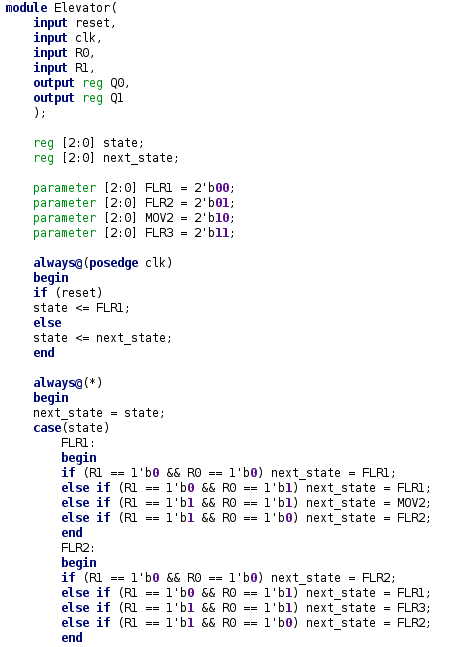
\includegraphics[width=0.8\textwidth]{State Machine Code 1.png}
        \end{minipage}
        \begin{minipage}{.5\textwidth}
            \centering
            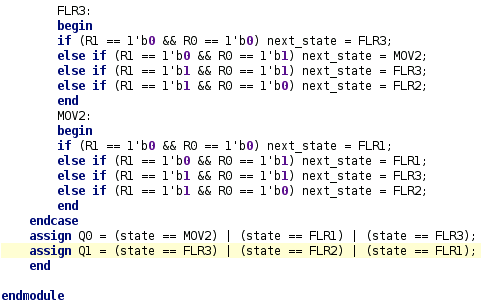
\includegraphics[width=0.9\textwidth]{State Machine Code 2.png}
        \end{minipage}
        \caption{State Machine Code}
    \end{figure}
    \par This is the code for the elevator controller within Verilog and a few
    things can be noticed. The first is that there are four inputs and two
    outputs. The outputs are designated as $Q_0$ and $Q_1$ and the inputs as,
    $R_0$, $R_1$, \textit{reset}, and \textit{clk}. The inputs $R_0$ and $R_1$
    are self-explanatory and they are the user inputs to the system. The other
    inputs however, are additional and are required for the functional operation
    of the machine. Since this is a state machine, the clock input is necessary
    as all state machines operate on a clock cycle. This particular machine
    operates on the positive edge of the clock, as seen by the \textit{always}
    block, argumented at \textit{posedge clk}.
    \par Here, the reset option is invoked and this input provides the sole
    purpose of "turning off" the machine. With the reset enabled the machine's
    state will go back to the first possible state, in this case $Q_0 Q_1 = 00$
    or, FLR1.
    \par From here, the design can be elaborated within Verilog and the
    schematic can be visualized. The schematic in this case is very unwieldy due
    to the fact that the elaboration does not seek to use the fewest number of
    gates to obtain the functionality. Despite this however, the function can be
    evaluated through the analysis of the waveform as done previously.
    \begin{figure}[h]
        \centering
        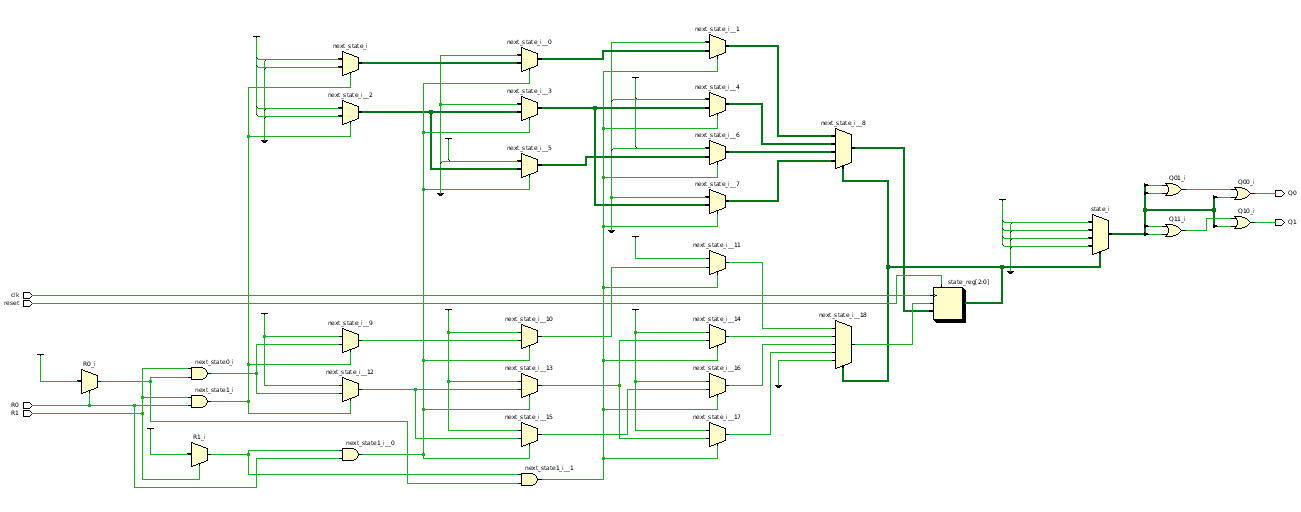
\includegraphics[width=0.8\textwidth]{State Machine Schematic.png}
        \caption{State Machine Schematic}
    \end{figure}
    \par This is the schematic generated and it can be seen that it is not what
    is really expected from the behavioral programming. Nevertheless, a
    simulation can be set up and the waveform will tell us if the device is
    working properly.
    \begin{figure}[h]
        \centering
        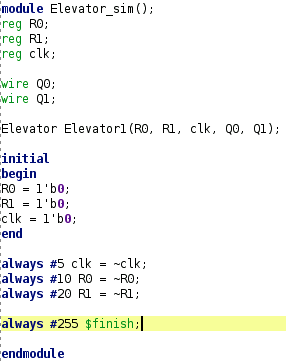
\includegraphics[width=0.3\textwidth]{State Machine Simulation Code.png}
        \caption{State Machine Simulation Code}
    \end{figure}
    \par Above is the code for the simulation of the created circuit. Here, the
    inputs and output can be seen as the user inputs and the clock, and the
    outputs $Q_0$ and $Q_1$. The "Elevator" module is instantiated and the given
    all the inputs and the corresponding outputs. The inputs are initialized as
    all zeros, and the simulation is ready to be started. In this screenshot of
    the code, the reset input is not present however, it must be known that the
    input was added after the fact and the waveform was constructed from there.
    The reset was taken as an input of the Elevator module as well and was
    responsible for proper starting of the machine.
    \begin{figure}[h]
        \centering
        \includegraphics[width=1.0\textwidth]{State Machine Waveform.png}
        \caption{State Machine Waveform}
    \end{figure}
    \par With the visualization of the waveform the reaction of the outputs with
    respect to the inputs can be seen. This shows how the machine works with the
    evolution of the clock and the user inputs and from the outputs, it can be
    seen that they are in correspondence with the transition table. Since the
    output cycle follows the state cycle defined in the table, the machine is
    working as intended and the implementation within Verilog is correct.
    \subsubsection*{Conclusion}
    \par This lab was fairly straight forward and was able to be done with
    simplicity as the transition table was given. The only real issue that was
    encountered was with the creation of the waveform as the outputs were not
    being represented correctly at first. This was an issue with the reset value
    as well and was eventually solved to form the proper waveform.  This lab was
    able to teach the design of a state machine from the ground up and
    exemplified how state machines actually achieve their function. It also
    discovers the reality of how state machines can be used to achieve a
    multitude of operations and how there ability to do so might be useful in
    many aspects of computing.
\end{document}
